
\documentclass{beamer}
\usecolortheme{dove}
\setbeamertemplate{navigation symbols}{}
\usepackage{amsmath,amssymb,amsfonts,amsthm, multicol, subfigure, color}
\usepackage{bm}
\usepackage{graphicx}
\usepackage{tabularx}
\usepackage{booktabs}
\usepackage{hyperref}
\usepackage{pdfpages}
\usepackage{xcolor}
\definecolor{seagreen}{RGB}{46, 139, 87}
\def\independenT#1#2{\mathrel{\rlap{$#1#2$}\mkern2mu{#1#2}}}
\newcommand\indep{\protect\mathpalette{\protect\independenT}{\perp}}
\def\log{\text{log}}
\newcommand\logit{\text{logit}}
\newcommand\iid{\stackrel{\text{iid}}{\sim}}
\newcommand\E{\text{E}}
\newcommand\V{\text{V}}
\renewcommand\P{\text{P}}
\newcommand{\Cov}{\text{Cov}}
\newcommand{\Cor}{\text{Cor}}
\newcommand\doop{\text{do}}
\usepackage{stackrel}
\usepackage{tikz}
\usetikzlibrary{arrows,shapes.arrows,positioning,shapes,patterns,calc}
\newcommand\slideref[1]{\vskip .1cm \tiny \textcolor{gray}{{#1}}}
\newcommand\red[1]{\color{red}#1}
\newcommand\blue[1]{\color{blue}#1}
\newcommand\gray[1]{\color{gray}#1}
\newcommand\seagreen[1]{\color{seagreen}#1}
\newcommand\purple[1]{\color{purple}#1}
\newcommand\orange[1]{\color{orange}#1}
\newcommand\black[1]{\color{black}#1}
\newcommand\white[1]{\color{white}#1}
\newcommand\teal[1]{\color{teal}#1}
\newcommand\magenta[1]{\color{magenta}#1}
\newcommand\Fuchsia[1]{\color{Fuchsia}#1}
\newcommand\BlueGreen[1]{\color{BlueGreen}#1}
\newcommand\bblue[1]{\textcolor{blue}{\textbf{#1}}}
\newcommand\bred[1]{\textcolor{red}{\textbf{#1}}}
\newcommand\bgray[1]{\textcolor{gray}{\textbf{#1}}}
\newcommand\bgreen[1]{\textcolor{seagreen}{\textbf{#1}}}
\newcommand\bref[2]{\href{#1}{\color{blue}{#2}}}
\colorlet{lightgray}{gray!40}
\pgfdeclarelayer{bg}    % declare background layer for tikz
\pgfsetlayers{bg,main} % order layers for tikz
\newcommand\mycite[1]{\begin{scriptsize}\textcolor{darkgray}{(#1)}\end{scriptsize}}
\newcommand{\tcframe}{\frame{
%\small{
\only<1|handout:0>{\tableofcontents}
\only<2|handout:1>{\tableofcontents[currentsubsection]}}
%}
}

\usepackage[round]{natbib}
\bibliographystyle{humannat-mod}
\setbeamertemplate{enumerate items}[default]
\usepackage{mathtools}

\title{1. Causal Questions: Observing and Intervening}
\author{Ian Lundberg\\Cornell Info 6751: Causal Inference in Observational Settings\\Fall 2022}
\date{23 Aug 2022}

\begin{document}

\maketitle

\section{Why causal inference?}

\begin{frame}{Why causal inference?}

What motivated you to take this course?

\end{frame}

\begin{frame}{Why causal inference?}

Why am I teaching this course? \pause \vskip .3in
Causal inference provides tools to
\begin{itemize}
\item Speak to policy interventions
\item Understand social systems
\end{itemize}

\end{frame}

\section{Central ideas for today}

\subsection{Causal claims hinge on arguments, not on data}

\begin{frame}
\tableofcontents
\end{frame}
\begin{frame}
\tableofcontents[currentsubsection]
\end{frame}

%\tcframe

\begin{frame}{Causal claims hinge on arguments, not on data}

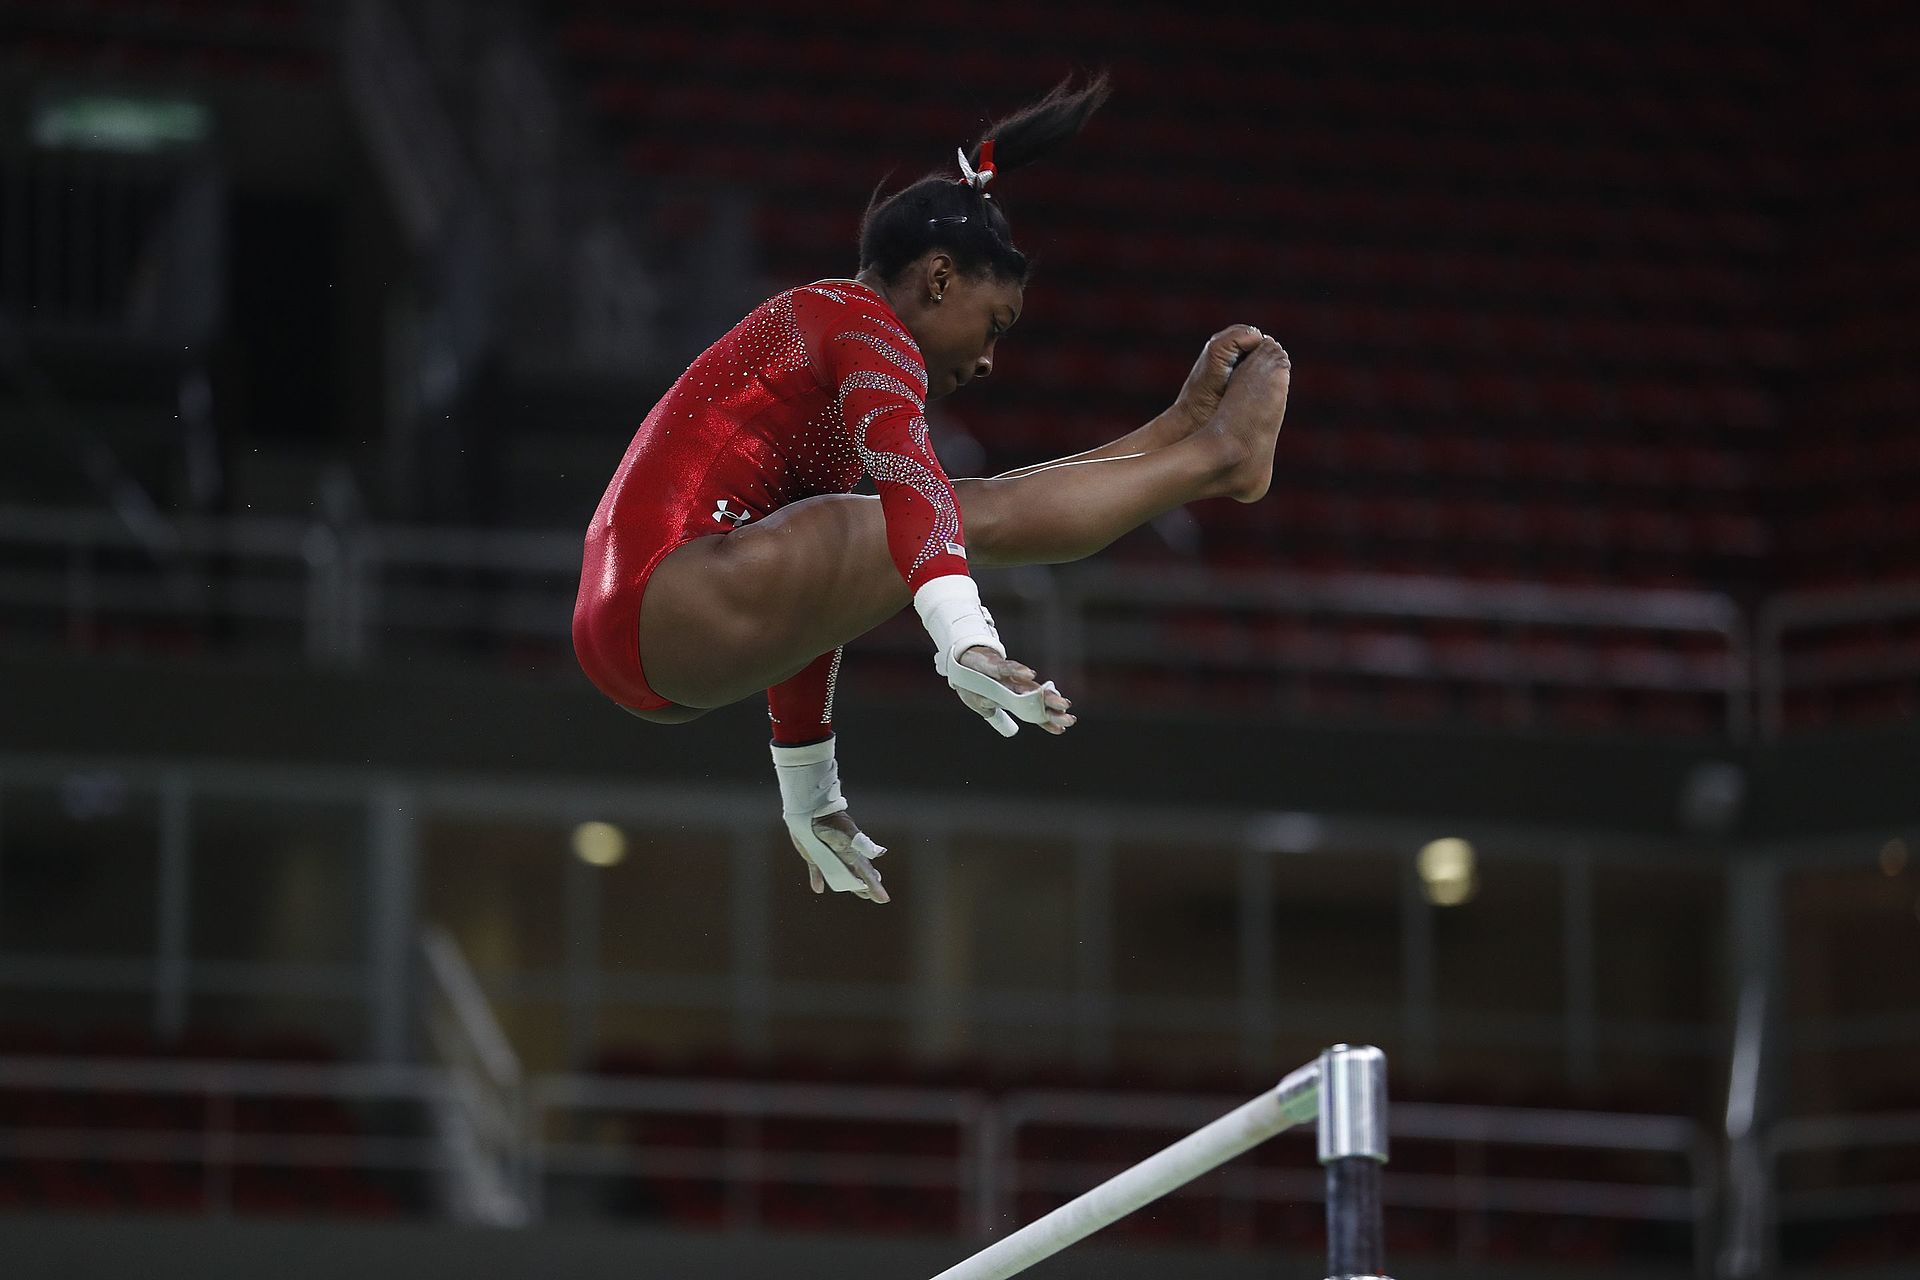
\includegraphics[width = .6\textwidth]{figures/Biles_bar}
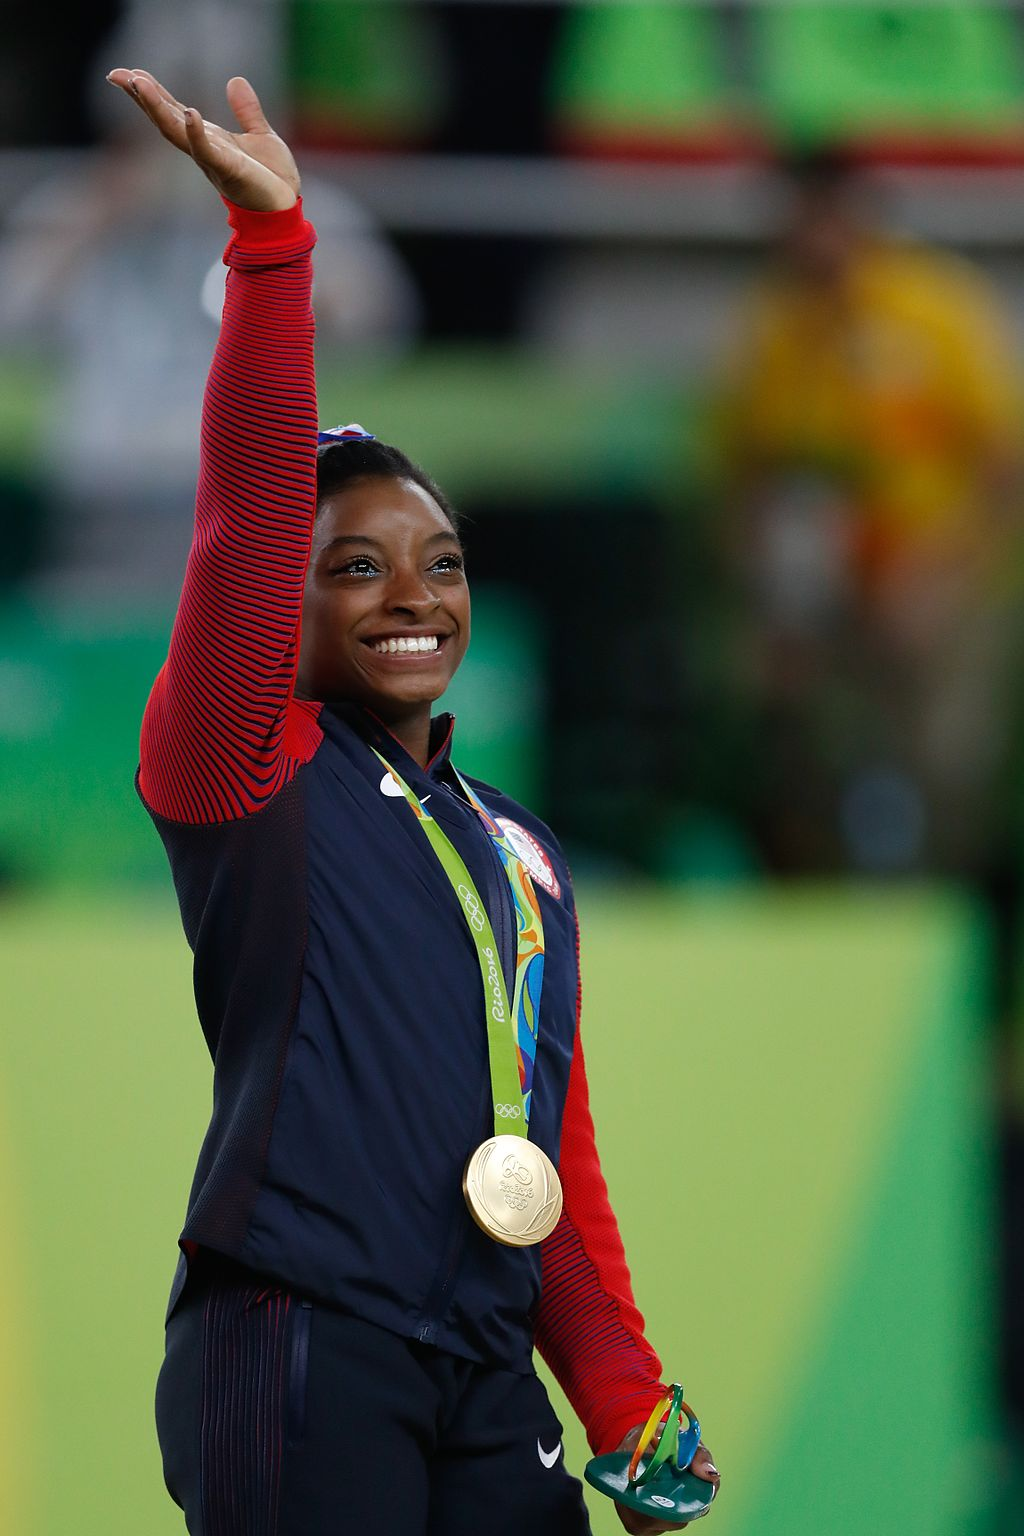
\includegraphics[width = .3\textwidth]{figures/Biles_medal}

\vskip .2in
\begin{tiny}
Left photo: By Fernando Frazão/Agência Brasil - \url{http://agenciabrasil.ebc.com.br/sites/_agenciabrasil2013/files/fotos/1035034-_mg_0802_04.08.16.jpg, CC BY 3.0 br, https://commons.wikimedia.org/w/index.php?curid=50548410} \\
Right photo: By Agencia Brasil Fotografias - EUA levam ouro na ginástica artística feminina; Brasil fica em 8 lugar, CC BY 2.0, \url{https://commons.wikimedia.org/w/index.php?curid=50584648}\\
\end{tiny}

\end{frame}

\begin{frame}{Causal claims hinge on arguments, not on data}
\begin{enumerate}
\item Statistical evidence
\begin{itemize}
\item Simone Biles swung on the uneven bars. She won a gold medal. \pause
\item I did not swing on the uneven bars. I did not win a gold medal.
\end{itemize} \pause
\item Possible causal claim
\begin{itemize}
\item Swinging on the uneven bars causes a person to win a gold medal.
\end{itemize}
\end{enumerate} \vskip .2in \pause
\begin{tabular}{rccc}
& \multicolumn{2}{l}{Do you win gold if you:} & Causal effect \\
& Swing & Do not swing & of swinging \\
\hline
Simone Biles & Yes (1) & \only<1-4>{?}\only<5->{\blue{No (0)}} & \only<1-5>{?}\only<6->{+1} \\
Ian & \only<1-6>{?}\only<7->{\blue{No (0)}} & No (0) & \only<1-7>{?}\only<8->{0} \\
\hline
\end{tabular}
\end{frame}

\subsection{Notation}

\subsubsection{Potential outcomes}

\tcframe

\begin{frame}{Notation: Potential outcomes}

\begin{tabular}{lll}
$Y_i$ & Outcome & Whether person $i$ won a gold medal \\
$A_i$ & Treatment & Whether person $i$ swung on the bars \\
$Y_i^a$ & Potential Outcome & Outcome person $i$ would realize if \\&&assigned to treatment value $a$
\end{tabular} \vskip .2in
\vskip .2in
Examples: \vskip .1in
\begin{footnotesize}
\begin{tabular}{rl}
$Y_\text{Biles} = 1$ & Simone Biles won gold \\
$A_\text{Biles} = 1$ & Simone Biles swung on the bars \\
$Y_\text{Biles}^1 = 1$ & If she swings, Simone Biles would win gold \\
$Y_\text{Biles}^0 = 0$ & If she does not swing, Simone Biles would not win gold
\end{tabular}
\end{footnotesize}

\end{frame}

\begin{frame}{Notation: Potential outcomes}
A person's potential outcomes are \bblue{deterministic mappings} \pause
\begin{itemize}
\item Simone Biles would win gold if she participates $Y_i^1 = 1$ \pause
\item Simone Biles would not win gold without participating $Y_i^0 = 0$
\end{itemize}
These are just numbers
\vskip .2in \pause
The outcome for a random person is a \bblue{random variable} \pause
\begin{itemize}
\item Draw a random person from the population \pause
\item Put them on the uneven bars \pause
\item The outcome $Y^1$ is a random variable:
\begin{itemize}
\item It takes the value 1 if we have sampled Simone Biles
\item It takes the value 0 if we have sampled anyone else
\end{itemize}
\end{itemize} \pause
We omit the subscript $i$ when talking about random people \vskip .1in \pause
\bgray{Check for understanding:}\\Does it make sense to write $\V(Y_i^1)$? How about $\V(Y^1)$

\end{frame}

\subsubsection{Consistency assumption}

\tcframe

\begin{frame}{Notation: The consistency assumption}
\begin{tikzpicture}[x = \textwidth, y = .8\textheight]
\draw[thick] (0,.6) -- (.4, .6) -- (.4,0);
\node[anchor = south] at (.2,0) {Potential Outcomes};
\node at (.1,.4) {$Y_i^1$};
\node at (.2,.4) {$Y_i^2$};
\node at (.15,.3) {$Y_i^3$};
\node at (.25,.3) {$Y_i^4$};
\onslide<2->{\draw[thick] (1,.6) -- (.6, .6) -- (.6,0);
\node[anchor = south] at (.8,0) {Factual Outcomes};
\node at (.8,.35) {$Y_i$};
}
\onslide<3->{
\node[anchor = south, align = center, blue, draw, rounded corners, line width = 1.2pt, inner sep = 12pt] at (.5,.65) {Consistency Assumption\\$Y_i^{A_i} = Y_i$};
}
\end{tikzpicture}
\end{frame}

\subsubsection{Expectation operator}

\tcframe

\begin{frame}{Notation: Expectation operator}
The \bblue{expectation operator} $\E()$ denotes the population mean
$$\E(Y^a) = \frac{1}{n}\sum_{i=1}^n Y_i^a$$
The quantity $Y^a$ inside the expectation must be a random variable \pause \vskip .6in
A \bblue{conditional expectation} is denoted with a vertical bar
$$\E(Y\mid A = a) = \frac{1}{n_a}\sum_{i:A_i=a} Y_i$$
\end{frame}

\subsubsection{Practicing notation}

\tcframe

\begin{frame}{Practice: How would you say this in English?}
\begin{enumerate}
\item $\E(\text{Earnings} \mid \text{Degree} = \texttt{TRUE}) > \E(\text{Earnings} \mid \text{Degree} = \texttt{FALSE})$
\onslide<2->{\begin{itemize}
\item Average earnings are higher among those with college degrees
\end{itemize}}\vskip .4in
\item $\E(\text{Earnings}^{\text{Degree} = \texttt{TRUE}}) > \E(\text{Earnings}^{\text{Degree} = \texttt{FALSE}})$ \vskip .1in
\onslide<3->{\begin{itemize}
\item On average, a degree causes higher earnings
\end{itemize}
}
\end{enumerate}
\end{frame}

\begin{frame}

A \bblue{descriptive} statement \hfill \begin{footnotesize} Language: among, disparity \end{footnotesize} \vskip .2in

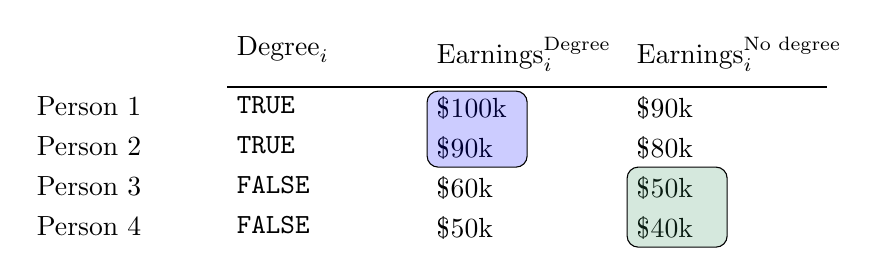
\begin{tikzpicture}[x = 1in, y = .2in]
\node[anchor = north west] (a) at (2,0.5) {$\text{Degree}_i$};
\node[anchor = north west] (d) at (3,0.5) {$\text{Earnings}_i^\text{Degree}$};
\node[anchor = north west] (nd) at (4,0.5) {$\text{Earnings}_i^\text{No degree}$};
\draw[thick] (2,-1) -- (5, -1);
\node[anchor = north west] (p2) at (1,-1) {Person 1};
\node[anchor = north west] (p2) at (1,-2) {Person 2};
\node[anchor = north west] (p3) at (1,-3) {Person 3};
\node[anchor = north west] (p4) at (1,-4) {Person 4};
\node[anchor = north west] (y11) at (2,-1) {\texttt{TRUE}};
\node[anchor = north west] (y21) at (2,-2) {\texttt{TRUE}};
\node[anchor = north west] (y31) at (2,-3) {\texttt{FALSE}};
\node[anchor = north west] (y41) at (2,-4) {\texttt{FALSE}};
\node[anchor = north west] (y11) at (3,-1) {\$100k};
\node[anchor = north west] (y21) at (3,-2) {\$90k};
\node[anchor = north west] (y31) at (3,-3) {\$60k};
\node[anchor = north west] (y41) at (3,-4) {\$50k};
\node[anchor = north west] (y10) at (4,-1) {\$90k};
\node[anchor = north west] (y20) at (4,-2) {\$80k};
\node[anchor = north west] (y30) at (4,-3) {\$50k};
\node[anchor = north west] (y40) at (4,-4) {\$40k};
\draw[fill opacity = .2, fill = blue, rounded corners] (3,-1.1) rectangle (3.5,-3);
\draw[fill opacity = .2, fill = seagreen, rounded corners] (4,-3) rectangle (4.5,-5);
\end{tikzpicture} 

\vskip .4in

A \bblue{causal} statement \hfill \begin{footnotesize}Language: effect, leads to, produces, benefits\end{footnotesize} \vskip .2in

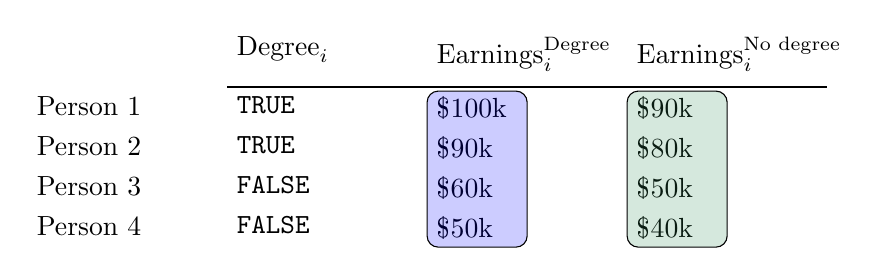
\begin{tikzpicture}[x = 1in, y = .2in]
\node[anchor = north west] (a) at (2,0.5) {$\text{Degree}_i$};
\node[anchor = north west] (d) at (3,0.5) {$\text{Earnings}_i^\text{Degree}$};
\node[anchor = north west] (nd) at (4,0.5) {$\text{Earnings}_i^\text{No degree}$};
\draw[thick] (2,-1) -- (5, -1);
\node[anchor = north west] (p2) at (1,-1) {Person 1};
\node[anchor = north west] (p2) at (1,-2) {Person 2};
\node[anchor = north west] (p3) at (1,-3) {Person 3};
\node[anchor = north west] (p4) at (1,-4) {Person 4};
\node[anchor = north west] (y11) at (2,-1) {\texttt{TRUE}};
\node[anchor = north west] (y21) at (2,-2) {\texttt{TRUE}};
\node[anchor = north west] (y31) at (2,-3) {\texttt{FALSE}};
\node[anchor = north west] (y41) at (2,-4) {\texttt{FALSE}};
\node[anchor = north west] (y11) at (3,-1) {\$100k};
\node[anchor = north west] (y21) at (3,-2) {\$90k};
\node[anchor = north west] (y31) at (3,-3) {\$60k};
\node[anchor = north west] (y41) at (3,-4) {\$50k};
\node[anchor = north west] (y10) at (4,-1) {\$90k};
\node[anchor = north west] (y20) at (4,-2) {\$80k};
\node[anchor = north west] (y30) at (4,-3) {\$50k};
\node[anchor = north west] (y40) at (4,-4) {\$40k};
\draw[fill opacity = .2, fill = blue, rounded corners] (3,-1.1) rectangle (3.5,-5);
\draw[fill opacity = .2, fill = seagreen, rounded corners] (4,-1.1) rectangle (4.5,-5);
\end{tikzpicture}

\end{frame}

\begin{frame}{Practice: How would you write this in math?}

\begin{enumerate}
\item On average, students who do the homework learn more than those who don't.
\onslide<2->{$$\E(\text{Learning}\mid \text{HW} = \texttt{TRUE}) > \E(\text{Learning}\mid \text{HW} = \texttt{FALSE})$$}
\item On average, doing the homework causes more learning.
\onslide<3->{$$\E(\text{Learning}^{\text{HW} = \texttt{TRUE}}) > \E(\text{Learning}^{\text{HW} = \texttt{FALSE}})$$}
\end{enumerate}

\end{frame}

\subsection{Fun example: Does A affect Y?}

\tcframe

\begin{frame}{Fun example: Does A affect Y?} \pause
\begin{tabular}{lll}
Treatment & $A_i$ & Receives heart transplant (1) vs. not (0) \\
Outcome & $Y_i$ & Dead (1) or alive (0) after five days
\end{tabular} \vskip .2in \pause
\begin{tabular}{lccl}
Unit & $Y_i^1$ & $Y_i^0$ & Causal Effect \\
\hline
Zeus & 0 & 1 & Transplant would save his life \\
Hera & 0 & 0 & Would survive regardless \\
Poseidon & 1 & 0 & Transplant would kill him \\
\hline
\end{tabular} \vskip .2in \pause
\bblue{Question:} Does a heart transplant cause death? \vskip .2in \pause

No. \\ The average causal effect is $\frac{1}{n}\sum_{i=1}^n \bigg(Y_i^1 - Y_i^0\bigg) = 1 + 0 - 1 = 0$ \vskip .1in \pause
Yes. \\ Potential outcomes are unequal. $Y_i^1\neq Y_i^0$ for at least some $i$
\end{frame}

\section{Logistics: Syllabus}

\begin{frame}
\tableofcontents
\end{frame}

\begin{frame}
\tableofcontents[currentsection]
\end{frame}

\begin{frame}{Syllabus: Learning goals\\\bref{https://tinyurl.com/Info6751}{tinyurl.com/Info6751}}
Students will learn to
\begin{itemize}
    \item evaluate the credibility of causal claims
    \item answer causal questions in their own research
    \item engage with new methods for causal inference
\end{itemize}
\end{frame}

\begin{frame}{Syllabus: Readings \\ \bref{https://tinyurl.com/Info6751}{tinyurl.com/Info6751}}
A combination of articles and this textbook: \vskip .2in
Hern\'an, M.A., and J.M. Robins. 2020. \emph{Causal Inference: What If?} Boca Raton: Chapman \& Hall / CRC. PDF available at \href{https://www.hsph.harvard.edu/miguel-hernan/causal-inference-book/}{hsph.harvard.edu/miguel-hernan/causal-inference-book/}
\end{frame}

\begin{frame}{Syllabus: Support \\ \bref{https://tinyurl.com/Info6751}{tinyurl.com/Info6751}}
\begin{itemize}
\item Ask questions on \bref{https://edstem.org/us/courses/26157/discussion/}{Ed Discussion}
\item Ask questions in office hours
\begin{itemize}
\item 1 hour after each class
\item \bref{https://calendly.com/ianlundberg/office-hours}{calendly.com/ianlundberg/office-hours}
\end{itemize}
\end{itemize}
\end{frame}

\begin{frame}{Syllabus: Assignments \\ \bref{https://tinyurl.com/Info6751}{tinyurl.com/Info6751}}
\begin{tabular}{lll}
1) Problem sets & Weekly & 50\% \\
2) Ideas for the research proposal & Oct 31 & 10\% \\
3) Final research proposal & Nov 21 & 30\% \\
4) Feedback to two peers & Dec 5 & 10\%
\end{tabular}
\end{frame}

\begin{frame}{Syllabus: Type and/or Handwrite \\ \bref{https://tinyurl.com/Info6751}{tinyurl.com/Info6751}}

I type math in \LaTeX.\\
You can type, handwrite, or combine the two. All equally good. \vskip .3in \pause

\bgray{Example.} A student thought about their expected happiness under an intervention to make them type math.\\
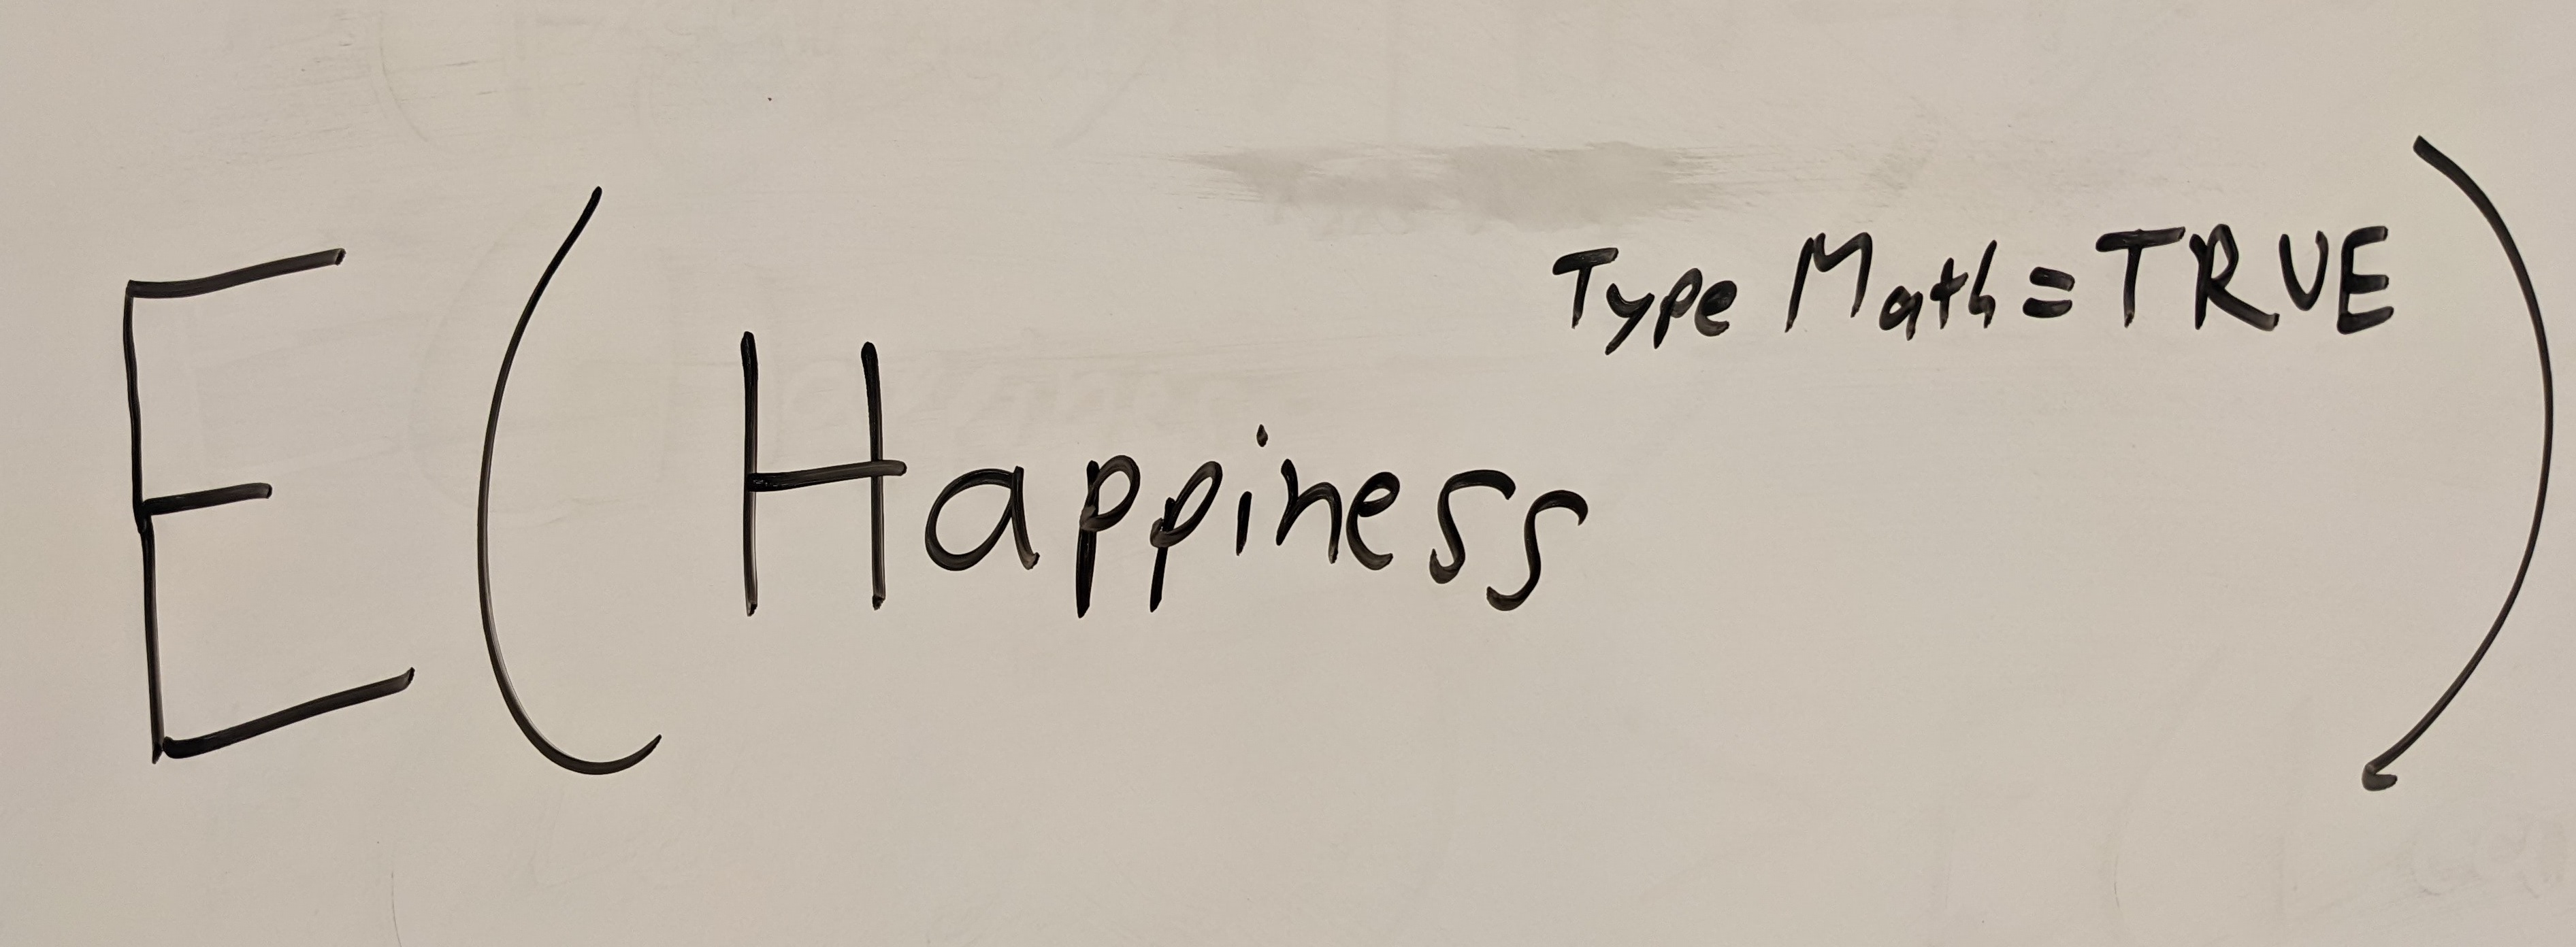
\includegraphics[width = .5\textwidth, trim = {2in 1in 0 0}, clip]{figures/type_math} \\
Then the student decided to handwrite.

\end{frame}

\begin{frame}{Syllabus: Suggested workflow \\ \bref{https://tinyurl.com/Info6751}{tinyurl.com/Info6751}}
Lecture $\rightarrow$ Reading $\rightarrow$ Problem Set \vskip .4in \pause
You are now ready to
\begin{itemize}
\item Read Hern\'an and Robins Ch 1
\item Complete Problem Set 1 Part 1
\end{itemize}
After Thursday, you will be ready to
\begin{itemize}
\item Read Hern\'an 2016
\item Complete Problem Set 1 Part 2
\end{itemize}
Problem set is due on Canvas Monday at 5pm
\end{frame}

\begin{frame}{Let me know what you are thinking}

\begin{huge} \bref{https://tinyurl.com/CausalQuestions}{tinyurl.com/CausalQuestions} \end{huge}
\vskip .7in

Office hours TTh 11am-12pm and at \bref{https://calendly.com/ianlundberg/office-hours}{calendly.com/ianlundberg/office-hours}\\Come say hi!

\end{frame}

\end{document}
